%% Ejemplo de la plantilla de latex para las diapositivas del Máster en IA 

%%%%%%%%%%%%%%%%%%%%%%%%%%%%
%% Valores para el ratio de aspecto: 43, 169 
%\documentclass[10pt, envcountsect, presentation, aspectratio=1610, hyperref={hypertexnames=true}]{beamer}
\documentclass[10pt, envcountsect, handout, aspectratio=1610, hyperref={hypertexnames=true}]{beamer}

%%%%%%%%%%%%%%%%%%%%%%%%%%%%

%%%%%%%%%%%%%%%%%%%%%%%%%%%%
%% Incluir fichero de estilo del máster
\input ../style/plantillaMasterIA.sty
%%%%%%%%%%%%%%%%%%%%%%%%%%%%

\addbibresource{../references.bib}



%\setbeameroption{show only notes} % Only notes
%\setbeameroption{show notes on second screen=right}  % Both
%\setbeamertemplate{note page}[compress]
\setbeameroption{hide notes} % Only slides



\renewcommand*\footnoterule{}
\setbeamerfont{footnote}{size=\tiny}




%\input{embed_video.tex}
%\usepackage{movie15}
\usepackage{multimedia}


%%%%%%%%%%%%%%%%%%%%%%%%%%%%
%% Información que aparecerá en la portada
\title[Aprendizaje por Refuerzo]{Aprendizaje por Refuerzo}
\subtitle{Programación Dinámica} % short title for footer

\author[L. D. Hernández] % Para el pie de página, poner los autores abreviados separados por comas.
{%
	\sc{Luis Daniel Hernández Molinero }\\ % Autor 1
	\textit{Ciencia de la Computación e Inteligencia Artificial}\\  % Area de conocimiento
	\textit{Dept. Ingeniería de la Información y las Comunicaciones}\\  % Departamento
	\\   % No dejes espacio entre esta línea y la llave siguiente 
}

\institute[DIIC]% % Poner las iniciales de los diferentes departamentos de los autores separadas por comas.
{
	\textit{Universidad de Murcia}
}

\newcounter{lastyear}
\setcounter{lastyear}{\the\year}
\addtocounter{lastyear}{-1}

\date{\arabic{lastyear} / \the\year} % Curso académico

%%%%%%%%%%%%%%%%%%%%%%%%%%%%%%%%%%
%% Contenido de las diapositivas
\setbeamerfont{normal text}{size=\normalsize} % Modifica el tamaño del texto de las diapositivas.
\AtBeginDocument{\usebeamerfont{normal text}}

%%%%%%%%%%%%%%%%%%%%%%%%%%%%%%%%%%

\begin{document}	

%%%%%%%%%%%%%%%%%%%%%%%%%%%%%%%%%%









%%%%%%%%%%%%%%%%%%%%%%%%%%%%%%%%%%

\begin{frame}[plain]
	\titlepage
\end{frame}

%%%%%%%%%%%%%%%%%%%%%%%%%%%%%%%%%%

\begin{frame}{Índice de Contenidos}
	\tableofcontents 

\end{frame}





%%%%%%%%%%%%%%%%%%%%%%%%%%%%%%%%%%
%%%%%%%%%%%%%%%%%%%%%%%%%%%%%%%%%%
\section{Introducción}

%%%%%%%%%%%%%%%%%%%%%%%%%%%%%%%%%%
%%%%%%%%%%%%%%%%%%%%%%%%%%%%%%%%%%
\begin{frame}{Introducción a la programación dinámica}

\scalebox{1.3}{
\begin{minipage}{.8\textwidth}
\begin{itemize}
\item\textbf{ ¿Qué es la programación dinámica?}  \citep{bellman1957dynamic}
    \begin{itemize}
        \item \key{Dinámica:} componente secuencial o temporal del problema.
        \item \key{Programación:} optimización de un "programa", como programación matemática.
    \end{itemize}

\item \key{Un método} para resolver problemas complejos:  
    \begin{itemize}
        \item \textbf{Descomponerlo} en subproblemas.
        \item \textbf{Resolver} los subproblemas.
        \item \textbf{Combinar} las soluciones de los subproblemas.
    \end{itemize}


\item \key{Ventajas} de la programación dinámica
    \begin{itemize}
        \item \textbf{Reutilización de subproblemas resueltos:} Evita resolver el mismo subproblema.
        \item \textbf{Optimalidad garantizada:} Si el problema cumple ciertas propiedades.
        \item \textbf{Aplicabilidad:} Se aplica a una amplia gama de problemas, como secuencias, optimización o grafos.
    \end{itemize}
\end{itemize}
\end{minipage}}

\end{frame}



%%%%%%%%%%%%%%%%%%%%%%%%%%%%%%%%%%
%%%%%%%%%%%%%%%%%%%%%%%%%%%%%%%%%%
\begin{frame}{Requisitos para la Programación Dinámica}
\scalebox{1.3}{
\begin{minipage}{.8\textwidth}
\begin{itemize}
\item \key{La programación dinámica es} es un método general para problemas con \textbf{dos propiedades}:
    \begin{itemize}
        \item \textbf{Estructura óptima de subproblemas:}  
        \begin{itemize}
            \item Aplica el \key{principio de optimalidad}.
            \item La solución óptima se obtiene de los óptimos de los subproblemas.
        \end{itemize}
        \item \textbf{Subproblemas superpuestos:}  
        \begin{itemize}
            \item Los subproblemas se repiten muchas veces.
            \item Memoización  y Tabulación: Las soluciones pueden almacenarse y reutilizarse en un orden \textit{ascendente}.
        \end{itemize}
    \end{itemize}

\centerline{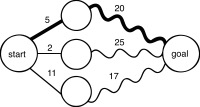
\includegraphics[width=.2\textwidth]{fig/Shortest_path_optimal_substructure}}


\item \key{Los procesos de decisión de Markov (MDP) satisfacen ambas propiedades:}  
    \begin{itemize}
        \item La ecuación de Bellman presenta una estructura óptima de subproblemas.
        \item La función de valor almacena y reutiliza soluciones.
    \end{itemize}
\end{itemize}
\end{minipage}}

\end{frame}


%%%%%%%%%%%%%%%%%%%%%%%%%%%%%%%%%%
%%%%%%%%%%%%%%%%%%%%%%%%%%%%%%%%%%
\begin{frame}{Planificación mediante programación dinámica}

\begin{itemize}
\item Diferencias clave entre \key{planificación} y \textbf{aprendizaje por refuerzo} (completo).

\hfil\scalebox{0.8}{\small
\begin{tabularx}{\textwidth}{|l|X|X|}
\hline
\textbf{Aspecto}               & \textbf{Planificación}                                     & \textbf{Aprendizaje por refuerzo completo}                    \\ \hline
\textbf{Conocimiento del MDP}   & Se conoce el MDP completo (\( P, R \)).              & El MDP es desconocido; el agente lo aprende al interactuar. \\ \hline
\textbf{Exploración}            & No es necesaria: el modelo ya es conocido.           & Es necesaria: el agente debe explorar para aprender el entorno. \\ \hline
\textbf{Técnicas principales}   & Programación dinámica, iteración de valor, iteración de política. &  Q-learning, SARSA, aprendizaje profundo. \\ \hline
\textbf{Objetivo}               & Resolver el MDP conocido (evaluar o controlar).      & Aprender la política óptima y las dinámicas del entorno. \\ \hline
\end{tabularx}
}

~



\item La Programación Dinámica se utiliza para la \key{planificación} en un MDP: 
\begin{itemize}
    \item Para \textbf{predicción}:  
    \begin{itemize}
        \item Entrada: MDP $\langle S,A,P,R, \gamma \rangle$ y política $\pi$.
        \item Salida: función de valor $v_\pi$: 
        $\ds
			v_\pi(s) = \mathbb{E}_\pi \left[ \sum_{t=0}^\infty \gamma^t R(s_t, a_t) \mid s_0 = s \right].
		$

    \end{itemize}
    \item Para \textbf{control}:  
    \begin{itemize}
        \item Entrada: MDP $\langle S,A,P,R, \gamma \rangle$.  
        \item Salida: función de valor óptima $v_*$ y política óptima $\pi^*$:
        $\ds
			v_*(s) = \max_\pi \mathbb{E}_\pi \left[ \sum_{t=0}^\infty \gamma^t R(s_t, a_t) \mid s_0 = s \right].
		$

    \end{itemize}
    
    \item La programación dinámica asume \key{conocimiento completo} del MDP. {\color{reddark} Ej:} Cubo Rubik vs Conducir  
\end{itemize}

\end{itemize}

\end{frame}




%%%%%%%%%%%%%%%%%%%%%%%%%%%%%%%%%%%%%%%%%%%%%%%%%%%%%%%%%%%%%%%%%%%%%%%%%%%%%%%%%%%%%%%%%%%%%%%%%%%%%%
%%%%%%%%%%%%%%%%%%%%%%%%%%%%%%%%%%%%%%%%%%%%%%%%%%%%%%%%%%%%%%%%%%%%%%%%%%%%%%%%%%%%%%%%%%%%%%%%%%%%%%
\section{Evaluación de Políticas (Predicción)}



%%%%%%%%%%%%%%%%%%%%%%%%%%%%%%%%%%
%%%%%%%%%%%%%%%%%%%%%%%%%%%%%%%%%%
\begin{frame}{Evaluación Iterativa de Políticas}

\begin{itemize}
\item 
\key{Problema (Predicción):} evaluar una política dada $\pi$. $\ds
			v_\pi(s) = \mathbb{E}_\pi \left[ \sum_{t=0}^\infty \gamma^t R(s_t, a_t) \mid s_0 = s \right].
		$
\item Podemos usar la expresión de las \key{ecuaciones de Bellman}:

$\ds v_\pi(s) = \sum_{a \in A} \pi(a|s) \left(R^a_s + \gamma \sum_{s' \in S} P^a_{ss'} v_\pi(s')\right)$\hfill 
$\ds v_\pi(s)   = \sum_{a\in\c{A}} \pi(a|s) \sum_{s',r} P_{ss'}^{ar} \left( R_s^a + \gamma v_\pi(s') \right)$

\item Tiene una expresión \key{matricial}: $\mbf{v}_\pi = \mbf{R}^\pi+ \gamma \mbf{P}^\pi \cdot \mbf{v}_\pi $ \;
	 
	\begin{itemize}
	\item $\mbf{v_\pi} = (\mbf{I} - \gamma \mbf{P}^\pi)^{-1} \mbf{R}^\pi$ (si invertible)
	\item Existencia y unicidad de $v_\pi$ si $\gamma < 1$ o temine
	\end{itemize}
	
\item \key{Otra solución:}  $\mbf{v_1} \to \mbf{v_2} \to \ldots \to \mbf{v_k} \to \ldots \stackrel{?}{\to} \mbf{v}_\pi$
	
\item \key{Actualizaciones basadas en expectativas} (o actualizaciones esperadas):  $\mbf{v}^\pi_{k+1} = \mbf{R}^\pi + \gamma \mbf{P}^\pi \mbf{v}_k$

$\ds v_{k+1}(s) = \sum_{a \in A} \pi(a|s) \left(R^a_s + \gamma \sum_{s' \in S} P^a_{ss'} v_k(s')\right)$\hfill 
$\ds v_{k+1}(s)   = \sum_{a\in\c{A}} \pi(a|s) \sum_{s',r} P_{ss'}^{ar} \left( R_s^a + \gamma v_k(s') \right)$

\item $v_\pi$ es un punto fijo {\color{reddark} \faArrowRight{}} Para $v_\pi$ la actualización esperada es la ecuación de Bellman
	\begin{itemize}
	\item Teorema: $\lim_{k\rightarrow \infty} v_k = v_\pi$
	\end{itemize}

\item ¡Tenemos algoritmo! Se llamará \key{evaluación iterativa de políticas}.
\end{itemize}

\end{frame}






%%%%%%%%%%%%%%%%%%%%%%%%%%%%%%%%%%
%%%%%%%%%%%%%%%%%%%%%%%%%%%%%%%%%%
\begin{frame}{Algoritmo: Evaluación iterativa de políticas}
\begin{minipage}{.9\textwidth}
\begin{algorithm}[H]
\caption{Evaluación Iterativa de Políticas para Estimar \(V \to v_\pi\)} \label{alg:EvalIteraPoliticas}
\begin{algorithmic}[1]
    \REQUIRE  $\pi$, la política a evaluar.  $\epsilon > 0$, un pequeño umbral, que determina la precisión de la estimación.
    \STATE INICIALIZAR $V(s)$ arbitrariamente para $s \in S$, y $V(\text{terminal}) = 0$.
    \REPEAT
        \STATE $\Delta \gets 0$
        \FOR{ $s \in S$}
            \STATE $v \gets V(s)$
            \STATE $\ds V(s) \gets \sum_{a} \pi(a|s) \sum_{s', r} p(s', r | s, a) [r + \gamma V(s')]$
            \STATE $\Delta \gets \max(\Delta, \; |v - V(s)|)$
        \ENDFOR
    \UNTIL{$\Delta < \epsilon$} \qquad \COMMENT{$\Delta = \max_{s \in S} |v_{k+1}(s) - v_k(s)| $}
\end{algorithmic}
\end{algorithm}
\end{minipage}
\end{frame}




%%%%%%%%%%%%%%%%%%%%%%%%%%%%%%%%%%
%%%%%%%%%%%%%%%%%%%%%%%%%%%%%%%%%%
\begin{frame}{Ejemplo: Pequeño mundo en cuadrícula}{Planteamiento del Problema}



\centerline{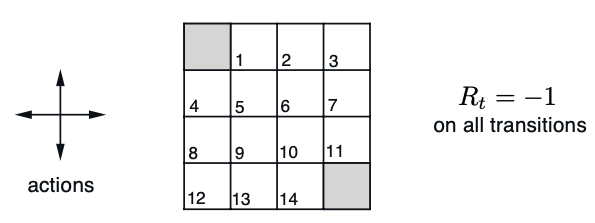
\includegraphics[width=0.6\linewidth]{fig/SmallWorld}}

~

\begin{itemize}
    \item Estados no terminales: 1, ..., 14.
    \item Un estado terminal (mostrado dos veces como cuadrados sombreados).
    \item Función de recompensa esperada: $r(s,a,s') = -1$ hasta que se alcance el estado terminal.
    \item MDP episódico no descontado ($\gamma = 1$).
    \item Las acciones que llevan fuera de la cuadrícula dejan el estado sin cambios.
    
    P.e, \(p(6, -1 | 5, \text{derecha}) = 1\), \(p(7, -1 | 7, \text{derecha}) = 1\), y \(p(10, r | 5, \text{a}) = 0\) para todo \(r \in R\) y $a \in A$.
    
    \item El agente sigue una política aleatoria equiprobable:  
    \[
    \pi(norte|\cdot) = \pi(este|\cdot) = \pi(sur|\cdot) = \pi(oeste|\cdot) = 0.25
    \]
\end{itemize}
\end{frame}



%%%%%%%%%%%%%%%%%%%%%%%%%%%%%%%%%%
%%%%%%%%%%%%%%%%%%%%%%%%%%%%%%%%%%
\begin{frame}{Ejemplo: Pequeño mundo en cuadrícula}{Evaluación Iterativa de Políticas}

	
\centerline{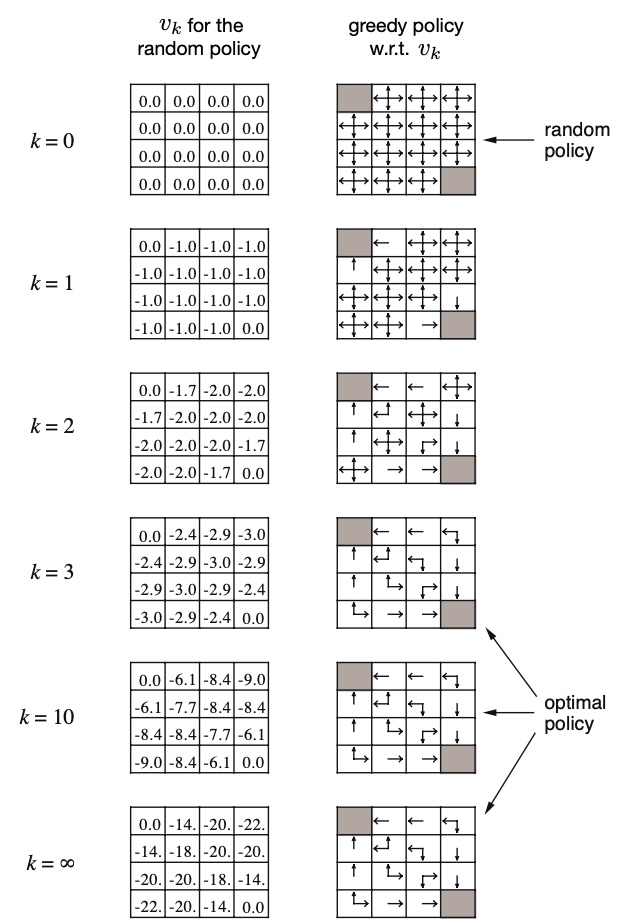
\includegraphics[width=0.5\linewidth, trim=0 440 0 0,clip]{fig/convergence_iterative_policy}
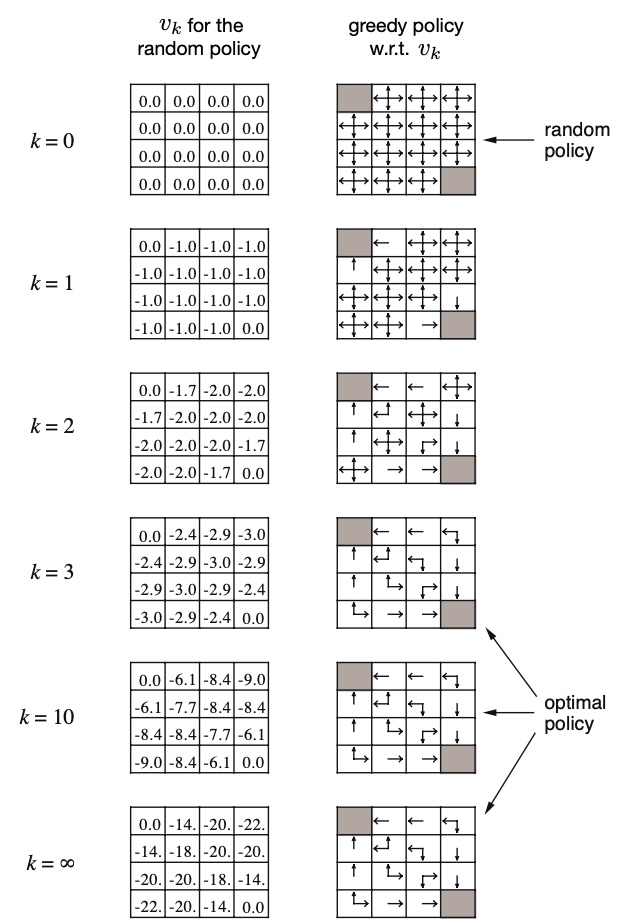
\includegraphics[width=0.5\linewidth, trim=0 0 0 500,clip]{fig/convergence_iterative_policy}}	

\vskip -0.25cm
		
\scriptsize
\begin{columns}
	\begin{column}{.5\textwidth}
		\begin{align*}
			v_1(s) & = \sum_{a \in A} \pi(a|s) \left[ R^a_s + \gamma \sum_{s' \in S} P^a_{ss'} v_0(s') \right] \\
			& = 4\cdot\frac{1}{4}\cdot [ -1 + 0 ]= -1
		\end{align*}
	\end{column}
	\begin{column}{.5\textwidth}
		
		\begin{align*}
			v_2(s) & = 0.25 \left[ -1 + v_1(s_{\text{Norte}}) \right] + 0.25 \left[ -1 + v_1(s_{\text{Sur}}) \right] \\
				   & + 0.25 \left[ -1 + v_1(s_{\text{Este}}) \right] + 0.25 \left[ -1 + v_1(s_{\text{Oeste}}) \right] = -2
		\end{align*}

		\vskip -1cm
		
		\begin{align*}
			v_2(s_T) & = 0.25 \left[ -1 + 0 \right] + 3 \times 0.25 \left[ -1 + (-1) \right] = -1.75
		\end{align*}
	

		
	\end{column}
\end{columns}

\end{frame}




%%%%%%%%%%%%%%%%%%%%%%%%%%%%%%%%%%
%%%%%%%%%%%%%%%%%%%%%%%%%%%%%%%%%%
\begin{frame}{Ejemplo: Pequeño mundo en cuadrícula}{¿Por qué mejora la política?}
	
	
\centerline{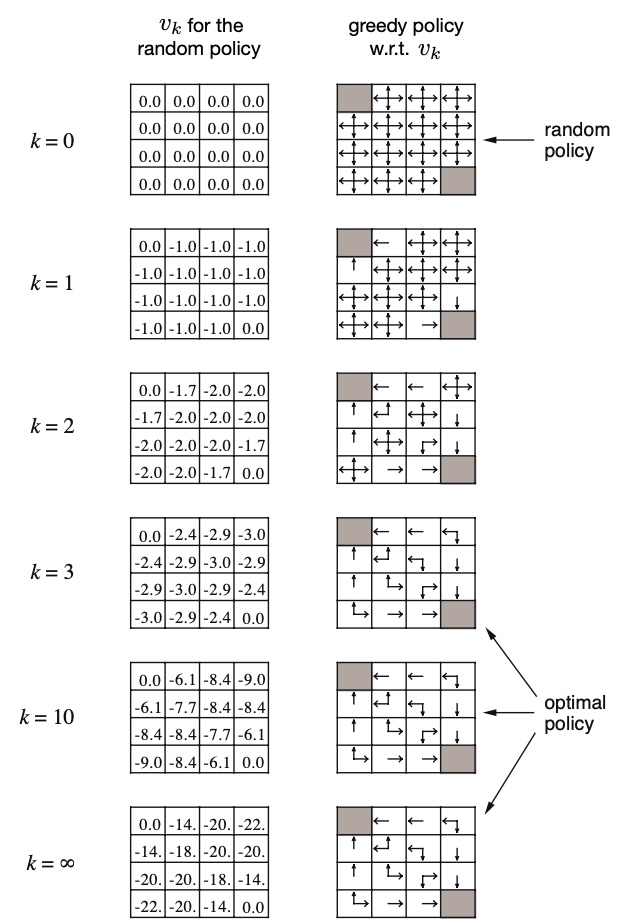
\includegraphics[width=0.5\linewidth, trim=0 440 0 0,clip]{fig/convergence_iterative_policy}
		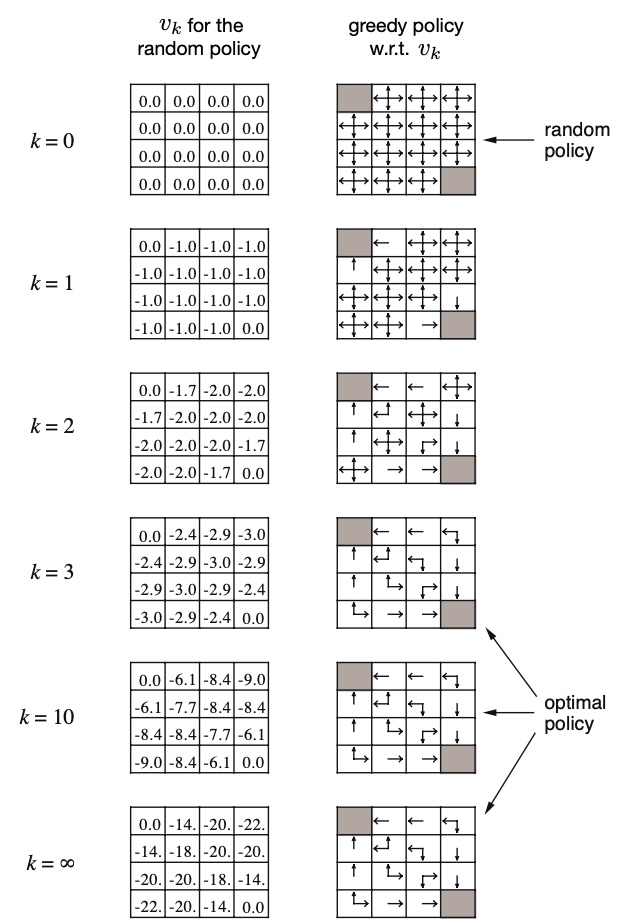
\includegraphics[width=0.5\linewidth, trim=0 0 0 500,clip]{fig/convergence_iterative_policy}}	

\vskip -0.25cm	
\scriptsize
\begin{columns}
	\begin{column}{.5\textwidth}
		\begin{align*}
			Q_k(s,a) & = R^{a}_s + \gamma \sum_{s'\in\c{S}} P^{a}_{ss'} v_k(s') \\
					 & =  R^{a}_s +  v_k(s')  \\
					 & (\gamma=1 \text{\ y \ } P^{a}_{ss'}=1)
		\end{align*}
	\end{column}
	\begin{column}{.5\textwidth}
		
		\begin{align*}
			s \text{\ adyacente a \ } s_T & \Rightarrow Q_2(s,a) =  R^{a}_s +  v_2(s_T) = -1 + 0 = -1 \text{\ (opt.)}\\
				   & \Rightarrow Q_2(s,a) =  R^{a}_s +  v_2(s') = -1  -2 = -3 \\
			s \text{\ esquina a \ } s_T & \Rightarrow Q_2(s,a) =  R^{a}_s +  v_2(s_T) = -1 -1.7= -2.7 \text{\ (opt.)}\\
				   & \Rightarrow Q_2(s,a) =  R^{a}_s +  v_2(s') = -1 - 2.0= -3
		\end{align*}
	

		
	\end{column}
\end{columns}	
\end{frame}





%
%%%%%%%%%%%%%%%%%%%%%%%%%%%%%%%%%%
%%%%%%%%%%%%%%%%%%%%%%%%%%%%%%%%%% 

\section{Mejorar la Política (Control)}


%%%%%%%%%%%%%%%%%%%%%%%%%%%%%%%%%%
%%%%%%%%%%%%%%%%%%%%%%%%%%%%%%%%%%
\begin{frame}{Mejora de Política}
	
	\begin{theorem}[Teorema de Mejora de Políticas Determinísiticas]
		Sean \(\pi\) y \(\pi'\)  dos política que verifican $q_\pi(s, \pi'(s)) \geq v_\pi(s)$  $\forall s \in S$,
		entonces:\\ 
		\hfil la política \(\pi'\) debe ser tan buena, o mejor que, \(\pi\): $v_{\pi'}(s) \geq v_\pi(s)$
	\end{theorem}
	
	\begin{itemize}
		\item Definimos una nueva \key{política determinística} o greedy: $\color{ForestGreen}\pi'(s) = \arg\max_a q_{\color{reddark}\pi}(s, a)$, por tanto  verifica:
		
		\hfil $ {\color{ForestGreen}\pi'}(s) = \arg\max_a q_\pi(s, a) =  \arg\max_a \sum_{s', r} p(s', r | s, a) \left[ r + \gamma v_{\color{reddark}\pi}(s') \right]$
		
		\item ¿\key{Será mejor} esta política determinística? \key{Sí}, porque:
		\begin{itemize}
			\item $\ds q_\pi(s, \pi'(s)) = \max_{a \in A} q_\pi(s, a) \Longrightarrow q_\pi(s, \pi'(s)) \geq q_\pi(s, a), \quad \forall a \in A$
			
			\item $\ds v_\pi(s) = \sum_{a \in A} \pi(a|s) q_\pi(s, a) \leq \max_{a \in A} q_\pi(s, a) = q_\pi(s, \pi'(s))$
			
			\item Por el teorema de mejora de políticas: $v_{\pi'}(s) \geq v_\pi(s)$ (es mejor)
			
		\end{itemize}

		\item Además: $\ds {\color{ForestGreen} v_{\pi'}}(s) = \max_{a\in \c{A}} q_\pi(s, a) = \max_{a\in \c{A}} \sum_{s', r} p(s', r | s, a) \left[ r + \gamma {\color{reddark} v_\pi}(s') \right]$, por ser codiciosa sobre $q_\pi()$
			
					
		\item \key{Durante el proceso:} llegamos a $\pi$, calculamos la nueva política codiciosa $\pi'$ y \key{ocurre que} $v_\pi = v_{\pi'}$, \textit{pues}:
		\begin{itemize}
			\item Se cumple la igualdad: $\ds {\color{reddark} v_{\pi'}}(s) = \max_{a\in \c{A}} q_{\color{reddark} \pi}(s, a) = \max_{a\in \c{A}} \sum_{s', r} p(s', r | s, a) \left[ r + \gamma {\color{reddark} v_{\pi'}}(s') \right]$
			\item Que se corresoponderá con \key{la ecuación de optimalidad de Bellman}: $\pi$ y $\pi'$ son $\pi_*$.
		\end{itemize}
		
		\item \key{Generalizando} a  $\pi(a|s)$ el T. de Mejora de Políticas se aplica tal cual. Si hay empates, distribuir $\color{reddark} \pi'$.
		
		
		
		
		
	\end{itemize}
	
\end{frame}






%
%%%%%%%%%%%%%%%%%%%%%%%%%%%%%%%%%%
%%%%%%%%%%%%%%%%%%%%%%%%%%%%%%%%%% 

\section{Iteración de Políticas}




%%%%%%%%%%%%%%%%%%%%%%%%%%%%%%%%%%
%%%%%%%%%%%%%%%%%%%%%%%%%%%%%%%%%% 

\subsection{Iteración de Políticas}

%%%%%%%%%%%%%%%%%%%%%%%%%%%%%%%%%%
%%%%%%%%%%%%%%%%%%%%%%%%%%%%%%%%%% 
\begin{frame}{Iteración de políticas}
\centerline{$\pi_0 \stackrel{E}{\longrightarrow} v_{\pi_0} \stackrel{I}{\longrightarrow} \pi_1 \stackrel{E}{\longrightarrow} v_{\pi_1} \stackrel{I}{\longrightarrow} \pi_2 \stackrel{E}{\longrightarrow} \dots \stackrel{I}{\longrightarrow} \pi_* \stackrel{E}{\longrightarrow} v_*,
$}
	

	
\begin{algorithm}[H]
	\caption{Iteración de políticas (usando evaluación iterativa de políticas) para estimar \(\pi \to \pi^*\)}
	
	\begin{enumerate}
		\item \textbf{Inicialización.} \hfil \(V(s) \in \mathbb{R}\) y \(\pi(s) \in {\cal A}(s)\) arbitrariamente para todo \(s \in {\cal S}\); \(V(\text{terminal}) = 0\)
		
		
		\item \key{Evaluación de la política.} \hfil Estimar $v_\pi$ mediante evaluación iterativa de políticas. \textbf{Algoritmo \ref{alg:EvalIteraPoliticas}}
					
		\item \key{Mejora de la política.} \hfil Generar $\pi' \geq \pi$ mediante una mejora codiciosa de la política.
		
		\vskip -1cm
		\begin{algorithmic}[1]
			\STATE \( {policy\text{-}stable} \leftarrow {True} \)
			\FOR{ \(s \in S\)}
			\STATE  \( \text{old-action} \leftarrow \pi(s) \)
			\STATE  \( \pi(s) \leftarrow \arg\max_a \sum_{s', r} p(s', r | s, a) [r + \gamma V(s')]\)
			\IF {\(\text{old-action} \not= \pi(s)\)}
			\STATE \( \text{policy-stable} \leftarrow \text{False} \)
			\ENDIF
			\ENDFOR
			\IF{\(\text{policy-stable}\)}
			\STATE detener y devolver \(V \to v^*\) y \(\pi \to \pi^*\); de lo contrario, volver a 2.
			\ENDIF
		\end{algorithmic}
		
	\end{enumerate}
\end{algorithm}

\end{frame}




%%%%%%%%%%%%%%%%%%%%%%%%%%%%%%%%%%
%%%%%%%%%%%%%%%%%%%%%%%%%%%%%%%%%% 
\begin{frame}{Ejemplo: Alquileres de coches}

\begin{itemize}
	\item \textbf{Estados:} Dos ubicaciones, con un máximo de 20 autos en cada una.
	\item \textbf{Acciones:} Mover hasta 5 autos entre las ubicaciones durante la noche.
	\item \textbf{Recompensa:} \$10 por cada auto alquilado (debe estar disponible). -\$2 por coche desplazado.
	\item \textbf{Transiciones:} Los autos son devueltos y solicitados de forma aleatoria.
	\begin{itemize}
		\item Distribución de Poisson: $n$ devoluciones/solicitudes con probabilidad $P(\lambda)=\ds \frac{\lambda^n}{n!}e^{-\lambda}$.
		\item Primera ubicación: solicitudes promedio = 3, devoluciones promedio = 3.
		\item Segunda ubicación: solicitudes promedio = 4, devoluciones promedio = 2.
	\end{itemize}
\end{itemize}


\centerline{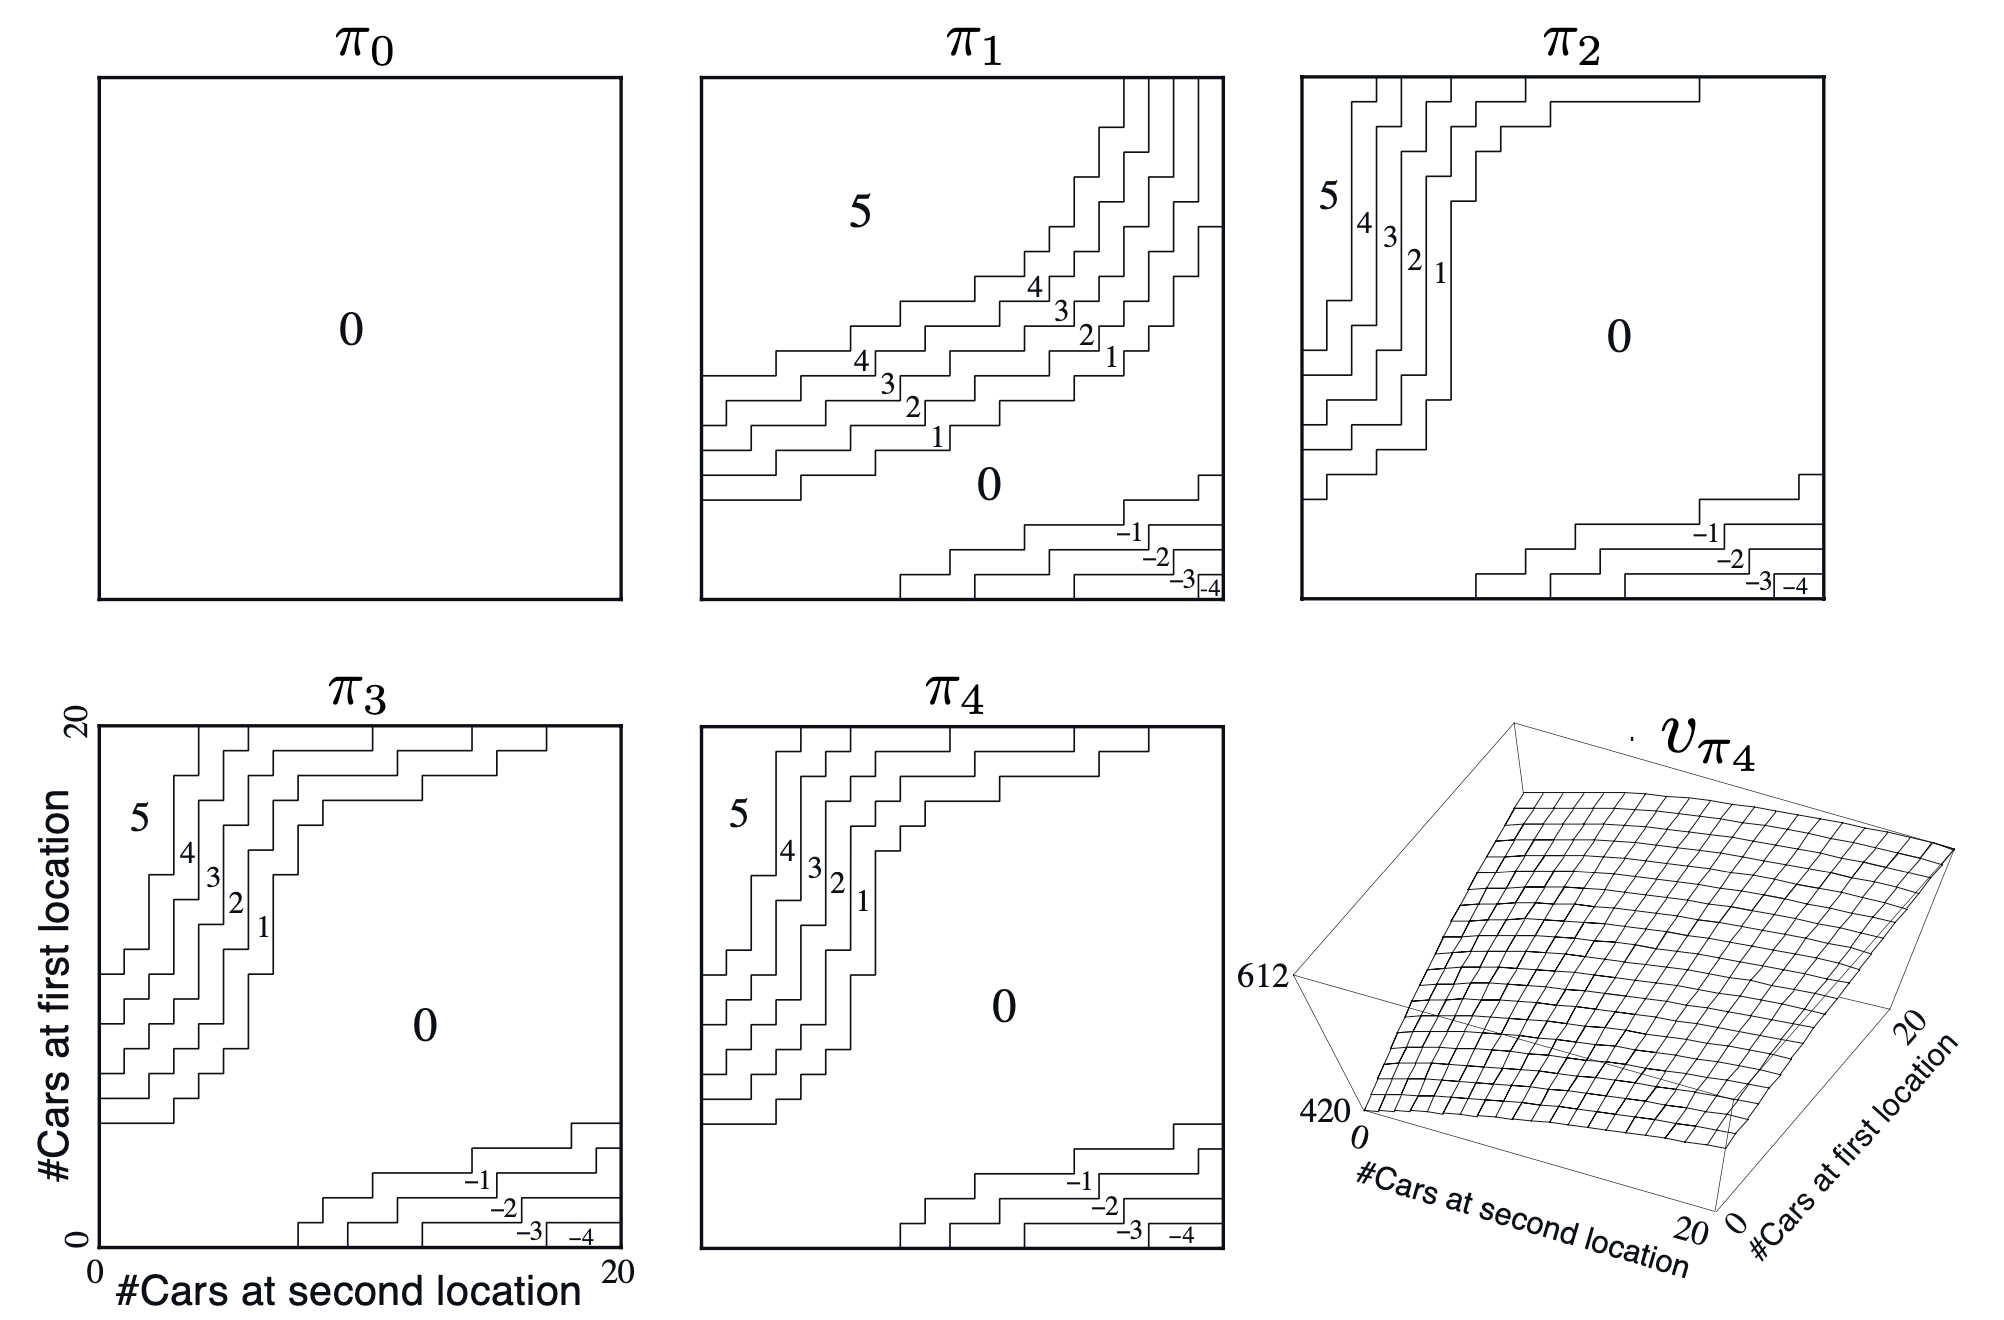
\includegraphics[width=.5\textwidth]{fig/jack_car_rental_example}}

%
\end{frame}







%%%%%%%%%%%%%%%%%%%%%%%%%%%%%%%%%%
%%%%%%%%%%%%%%%%%%%%%%%%%%%%%%%%%%
\begin{frame}{Iteración de Políticas Modificada}
\begin{itemize}
	\item \key{Iteración de Políticas Clásica}: Repite los siguientes pasos 1 y 2 hasta que no cambia $\pi$
		\begin{enumerate}
			\item \key{Evaluación de políticas:}
			$
			v_\pi(s) = \sum_{a \in A} \pi(a \mid s) \left[ R^a_s + \gamma \sum_{s' \in S} P^a_{ss'} v_\pi(s') \right].
			$
			
			\begin{itemize}
				\item $\ds v_{k+1}(s) = \sum_{a \in A} \pi(a|s) \left(R^a_s + \gamma \sum_{s' \in S} P^a_{ss'} v_k(s')\right)$
				\item Teorema: $\lim_{k\rightarrow \infty} v_k = v_\pi$
				\item En la práctica $|v_{k+1}-v_{k}|<\epsilon$
			\end{itemize}
				
			\item \key{Mejora de políticas (greedy):} 
			\(
			\pi'(s) = \arg\max_a \left[ R^a_s + \gamma \sum_{s' \in S} P^a_{ss'} v_\pi(s') \right].
			\)
			
		\end{enumerate}
		
	\item \key{Algunas preguntas}. En algunos problemas llagamos antes a la política óptima, entonces ...
	\begin{itemize}
	    \item ¿Es necesario que la evaluación de políticas converja completamente a $v_\pi$?
	    \item ¿O debería introducirse una condición de parada (e.g., convergencia $\epsilon$ de la función de valor)?
	    \item ¿O simplemente detenerse después de $k$ iteraciones de evaluación iterativa de políticas?
	\end{itemize}
	
	\item Un algoritmo de \key{Iteración de Políticas Modificada} \citep{puterman1978modified} es cualquier algoritmo que realice la evaluación de políticas un número finito de veces $k=1, 2, \ldots, \infty$.
\end{itemize}
\end{frame}



%
%%%%%%%%%%%%%%%%%%%%%%%%%%%%%%%%%%
%%%%%%%%%%%%%%%%%%%%%%%%%%%%%%%%%% 

\subsection{Iteración  de Políticas Generalizada}


%%%%%%%%%%%%%%%%%%%%%%%%%%%%%%%%%%
%%%%%%%%%%%%%%%%%%%%%%%%%%%%%%%%%%
\begin{frame}{Iteración  de Políticas Generalizada}
	\begin{columns}
		\begin{column}{.5\textwidth}
			\hfil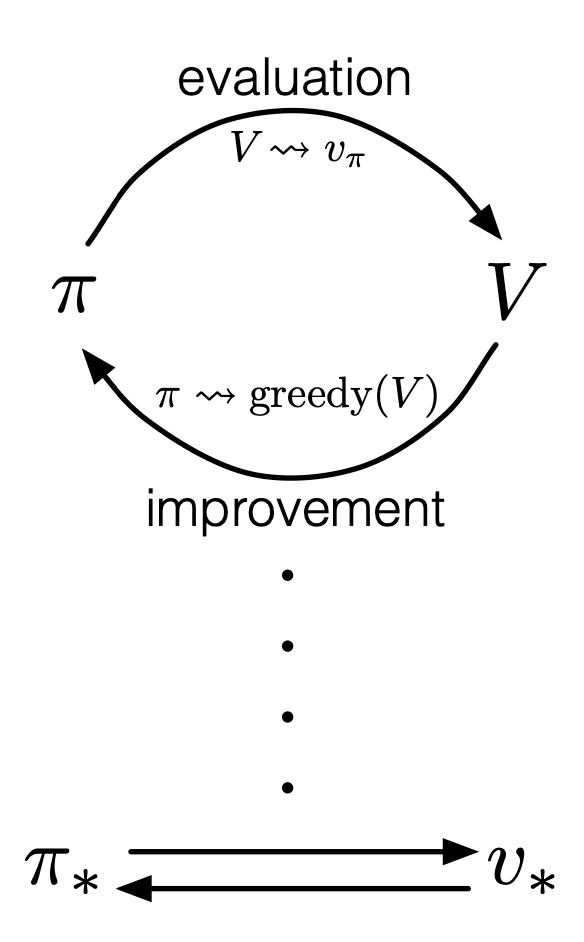
\includegraphics[width=.5\textwidth]{fig/iteracion_generalizada}
			\begin{itemize}
				\item			 Ambos procesos se estabilizan cuando se encuentra una política que es codiciosa con respecto a su propia función de evaluación
			\end{itemize}
		\end{column}
		\begin{column}{.5\textwidth}
			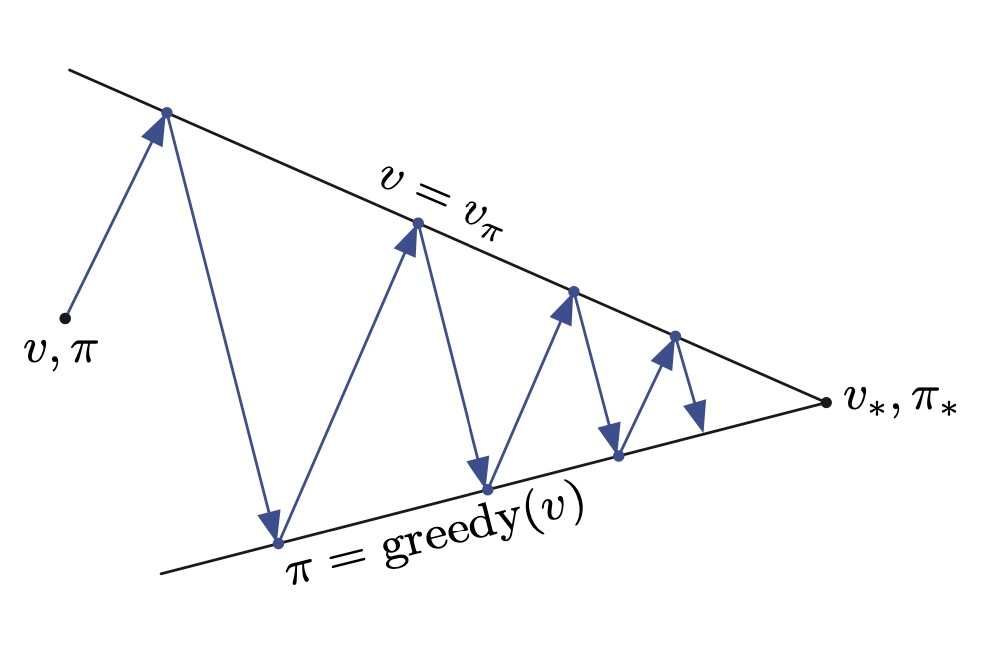
\includegraphics[width=.8\textwidth]{fig/iteracion_generalizada2}
			
			~
			
			\begin{itemize}
				\item \textbf{Evaluación de política} {Estimar } $v_\pi$
					\begin{itemize}
						\item \textcolor{reddark}{Cualquier algoritmo} de evaluación  de política
					\end{itemize}
				\item \textbf{Mejora de política} Generar  $\pi' \geq \pi$
					\begin{itemize}
						\item \textcolor{reddark}{Cualquier algoritmo} de \textbf{mejora} de política
					\end{itemize}
			\end{itemize}			
		\end{column}	
	\end{columns}

\end{frame}



%%%%%%%%%%%%%%%%%%%%%%%%%%%%%%%%%%
%%%%%%%%%%%%%%%%%%%%%%%%%%%%%%%%%% 

\subsection{Iteración de Valor}


%%%%%%%%%%%%%%%%%%%%%%%%%%%%%%%%%%
%%%%%%%%%%%%%%%%%%%%%%%%%%%%%%%%%%
\begin{frame}{Principio de optimalidad}
	
	\begin{itemize}
		\item La optimalidad de un problema NO viene dado por la optimalidad de sus subproblemas.
		
		\begin{itemize}
			\item $\max x + y$ s.a.  $x + y \leq 1$ con $x, y \in \{0, 1\}$
			
			Tiene soluciones óptimas \( (0, 1) \) y \( (1, 0) \). Ambas suman 1.
			
			\item Subproblema 1. Maximizar \( x \) con $x \in \{0, 1\}$. Solución óptima: \( x = 1 \)
			\item Subproblema 2. Maximizar \( y \) con $y \in \{0, 1\}$. Solución óptima: \( y = 1 \)
			\item La composición de soluciones parciales $x+y=1+1=2$ ni siquiera cumple las restricciones.
		\end{itemize}

	
		\item \begin{minipage}{.9\textwidth}
			\begin{block}{Principio de Optimalidad}
				Una política óptima tiene la propiedad de que cualquiera que sea el estado inicial y la decisión inicial, las decisiones restantes deben constituir una política óptima en relación con el estado resultante de la primera decisión. \citep{bellman1957dynamic}
			\end{block}
		\end{minipage}
		
			~
			
			\begin{itemize}
				\item Si una solución es óptima, las subsoluciones son óptimas.
			\end{itemize}
	
		\item \begin{minipage}{.9\textwidth}
			\begin{theorem}[Principio de Optimalidad]
				Una política $\pi(a|s)$ alcanza el valor óptimo desde el estado $s$, $v_\pi(s) = v^*(s)$, si y solo si:  
				\begin{itemize}
					\item Cualquier estado $s'$ es alcanzable desde $s$ de forma óptima.
					\item $\pi$ alcanza el valor óptimo desde el estado $s'$, $v_\pi(s') = v^*(s')$.
				\end{itemize}
			\end{theorem}
\end{minipage}

\end{itemize}	

\end{frame}






%%%%%%%%%%%%%%%%%%%%%%%%%%%%%%%%%%
%%%%%%%%%%%%%%%%%%%%%%%%%%%%%%%%%%
\begin{frame}{Iteración de valores determinista}
\begin{columns}
	\begin{column}{.4\textwidth}

	\begin{tikzpicture}[
		%scale=1.0,
		> = {Latex[width=4pt,length=8pt]},  % estilo de flecha
		%every path/.style = {line width=1pt}  % grosor para todos los paths
		state/.style={circle, draw, scale=10, inner sep=0},
		action/.style={circle, fill=black,  scale=5, inner sep=0},
		every node/.style={font=\scriptsize}
		]
		
		% Nodes
		\node[state] (s) at (0,0) {};
		\node (pi) at (0,-0.5) {$\pi(a|s)$};
		\node[action] (a1) at (-1.5,-1) {};
		\node[action] (a2) at (1.5,-1) {};
		\node[state] (s11) at (-2.5,-2.2) {};
		\node[state] (s12) at (-0.5,-2.2) {};
		\node[state] (s21) at (0.5,-2.2) {};
		\node[state] (s22) at (2.5,-2.2) {};
		
		
		
		% Arrows
		\draw[->] (s) -- (a1);
		\draw[->] (s) -- (a2);
		
		\draw[->] (a1) --  node[left, yshift=1mm] {$r$} (s11) ;
		\draw[->] (a1) -- (s12);
		\draw[->] (a2) -- (s21);
		\draw[->] (a2) -- (s22);
		
		% Additional labels
		\node[left] at (s.west) {$v_*(s) \leftarrow s$};
		\node[left] at (a1.west) {$a_1=a^*$};
		\node[left] at (a2.west) {$a_2$};
		\node[left] at (s11.west) {$v_*(s')$};
		\node[left] at (s12.west) {$v_*(s')$};		
	\end{tikzpicture}
	\end{column}
	
	\begin{column}{.5\textwidth}
		Si una trayectoria es óptima debe estar compuesta por subtrayectorias óptimas.
		
		~\hfill \textit{-- Principio de Optimalidad}
	\end{column}
	
\end{columns}	
\begin{itemize}
	\item Para \key{garantizar el principio de optimalidad}, cualquier política óptima debe poder subdividirse en dos componentes:  
	\begin{itemize}
		\item Una acción inicial óptima $a^*$.
		\item Seguido de una política óptima desde sus estados sucesores $S'$ (porque necesitamos un valor esperado).
	\end{itemize}
	

	\item Si conocemos la solución a los subproblemas $v_*(s')$,  entonces la solución $v_*(s)$ se puede encontrar mediante una \key{evaluación de un paso}:  
		\[
		v^*(s) \leftarrow \max_{a \in A} \left(R^a_s + \gamma \sum_{s' \in S} P^a_{ss'} v^*(s')\right)
		\]
		\textbf{Idea:} aplicar estas actualizaciones de manera iterativa.  
		\begin{itemize}
		    \item Intuición: Comenzar con las recompensas finales y trabajar hacia atrás.
		    \item Funciona incluso con MDPs estocásticos y con bucles.
		\end{itemize}
\end{itemize}

\end{frame}

%%%%%%%%%%%%%%%%%%%%%%%%%%%%%%%%%%
%%%%%%%%%%%%%%%%%%%%%%%%%%%%%%%%%%
\begin{frame}{Ejemplo: Camino más corto - I}{$v_{k+1}(s) \leftarrow \max_{a \in A} \left[ R(s,a) + \gamma \sum_{s'} P(s'|s,a) v_k(s') \right]$ \tiny $= \max_{a \in A} \left[ R(s,a) +  v_k(s') \right]$}
\centerline{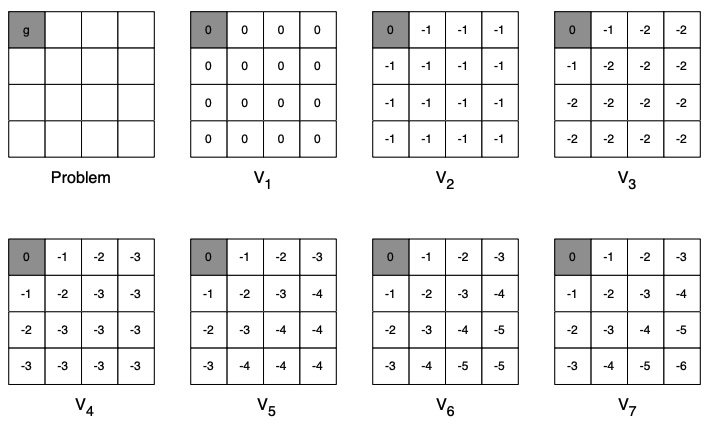
\includegraphics[width=0.8\linewidth, trim=0 240 0 0,clip]{fig/ShortPath}
}

\begin{itemize}
	\item Problema: Encontrar el camino más corto hasta el objetivo \textbf{g}. $R(s,a) = -1$ y $\gamma=1$
	\item $v_1$. Definimos $v_1(s)=0$ $\forall s$
	\item $v_2$. \scalebox{1.1}{$\Bigg\{$}
	\begin{minipage}{.8\textwidth}
		\begin{itemize}
				\item Estado terminal $(1,1)$: {\small $v_1(1,1) = v_0(1,1) = 0$}. No hay acciones
				\item Estados no terminales {\footnotesize $(i,j) \not =  (1,1)$. $v_1(i,j) = \max_a [R_s^a + \sum_{s'} P(s'|s,a) v_0(s')] = -1+0 = -1$}.
		\end{itemize}
	\end{minipage}
	
	
\item $v_2$. \scalebox{1.5}{$\Bigg\{$}
	\begin{minipage}{.8\textwidth}
		\begin{itemize}
			\item Estado terminal $(1,1)$: $v_2(1,1) = v_1(1,1) = 0$. No hay acciones
			\item Adyacentes al terminal $v_2(i,j) = \max_a [R_s^a + \sum_{s'} P(s'|s,a) v_1(s')] = \max\{-1, -2\} = -1$.
			\item Resto de estados: $	v_{2}(s) = \max_{a \in A} [ -1 + v_1(s') ] = \max{-2} =-2$
		\end{itemize}
	\end{minipage}
\end{itemize}

\end{frame}




%%%%%%%%%%%%%%%%%%%%%%%%%%%%%%%%%%
%%%%%%%%%%%%%%%%%%%%%%%%%%%%%%%%%%
\begin{frame}{Ejemplo: Camino más corto - II}{$v_{k+1}(s) \leftarrow \max_{a \in A} [ -1 + v_k(s') ]$}
	\centerline{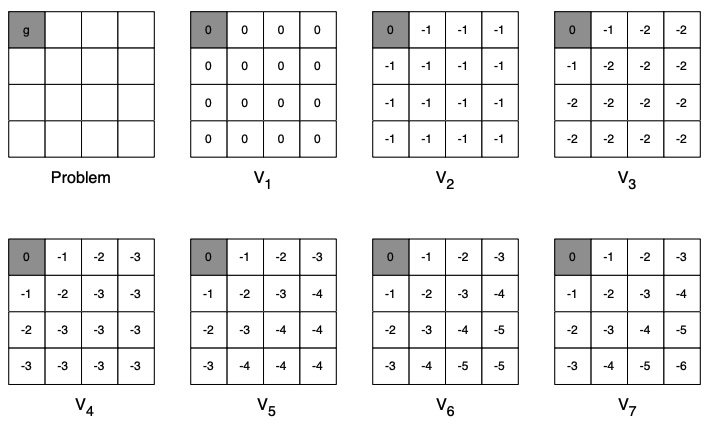
\includegraphics[width=0.8\linewidth]{fig/ShortPath}}
	

	
	\note<1>{
		\begin{itemize}
			\item La evolución de las evaluaciones se muestran en esta transaparencia.

			\item En este ejemplo se tiene que la expresión con la que actualiza $v_{k+1}(s)$ que es  $\max_{a \in A} \left[ R(s,a) + \gamma \sum_{s'} P(s'|s,a) v_k(s') \right]$ se reduce a calcular el valor $v_{k+1}(s) \leftarrow \max_{a \in A} [ -1 + v_k(s') ]$, que se encuentra en el título de la transparencia.
			
			\item Podéis comprobar los valores de cada evaluación $V_{k+1}$ usando esa fórmula tan simple.
			
			\item A partir de la evaluación $V_7$ las evaluaciones no cambian.
			
			\item Y vemos que los valores se corresponde con el número de pasos que habría que realizar para llegar al objetivo si nos movemos como una torre del ajedrez a un solo paso.
			
			
		\end{itemize}
		\fin
	}	
	
\end{frame}




%%%%%%%%%%%%%%%%%%%%%%%%%%%%%%%%%%
%%%%%%%%%%%%%%%%%%%%%%%%%%%%%%%%%%
\begin{frame}{Iteración de valores}


\begin{algorithm}[H]
	\caption{Iteración de valor para estimar \(V \to v^*\)}
	\begin{algorithmic}[1]
		\REQUIRE Un pequeño umbral \(\epsilon > 0\) que determina la precisión de la estimación.
		\STATE Inicializar \(V(s)\), para todo \(s \in S^+\), arbitrariamente excepto que \(V({terminal}) = 0\).
		\REPEAT
		\STATE \(\Delta \leftarrow 0\)
		\FOR{cada \(s \in S\)}
		\STATE \(v \leftarrow V(s)\)
		\STATE \(\ds V(s) \leftarrow \max_a \sum_{s', r} p(s', r | s, a) \left[ r + \gamma V(s') \right]\)
		\COMMENT{Alternativamente $\ds \max_{a \in A} \left(R^a_s + \gamma \sum_{s' \in S} P^a_{ss'} v_k(s')\right)$}
		\STATE \(\Delta \leftarrow \max(\Delta, |v - V(s)|)\)
		\ENDFOR
		\UNTIL{ \(\Delta < \epsilon\)  }
		\ENSURE  una política determinista, \(\pi \approx \pi^*\), tal que 
		\(\pi(s) = \ds \arg\max_a \sum_{s', r} p(s', r | s, a) \left[ r + \gamma V(s') \right]\)
	\end{algorithmic}
\end{algorithm}

\end{frame}




%%%%%%%%%%%%%%%%%%%%%%%%%%%%%%%%%%
%%%%%%%%%%%%%%%%%%%%%%%%%%%%%%%%%%
\begin{frame}{Iteración de valor: Lo mires por donde lo mires}
\begin{itemize}
	\item[]\quad 	
	\textbf{La siguiente expresión}  \key{se obtiene por distintos criterios}:
	
	
$$\ds v(s) \leftarrow \max_a \sum_{s', r} p(s', r | s, a) \left[ r + \gamma v(s') \right] \qquad \qquad
\mbf{v} \leftarrow \max_a \left[ \mbf{R}^a + \gamma \mbf{P}^a \mbf{v} \right]
$$
	



	\item \key{El principo de optimalidad.}
		\begin{itemize}
			\item Explicación anterior
		\end{itemize}
		
	\item \key{Ecuación de optimalidad de Bellman.}	$\ds v_*(s) = \max_a \sum_{s', r} p(s',r|s,a) \left(r + \gamma v_*(s') \right]	$
			
		\begin{itemize}
		\item El algoritmo aplica una evaluación iterativa sobre la ecuación de optimalidad 
		\end{itemize}
		
	\item \key{Iteración de política modificada.}
	\begin{itemize}
		\item Iteración de política modificada: \textbf{una} evaluación de la función valor y después cambia a política greedy.
			\begin{itemize}
				\item $\ds {\color{ForestGreen} v_{\pi'}}(s) = \max_{a\in \c{A}} \sum_{s', r} p(s', r | s, a) \left[ r + \gamma {\color{reddark} v_\pi}(s') \right] = $
				\begin{minipage}{.5\textwidth}
					$ \ds
					\left\{
					\begin{array}{l}
						 1. \ds v_{\pi}(s)  \leftarrow \sum_{a\in\c{A}} \pi(a|s) \sum_{s',r}  p(s',r|s,a) \left( r + \gamma {\color{reddark} v_\pi}(s') \right) \\
						 2. \ds {\color{ForestGreen} v_{\pi'}}(s) = \max_{a\in \c{A}} q_\pi(s, a)
					\end{array}
					\right.
					$
				\end{minipage}
			\end{itemize}
			
			
	\end{itemize}
\end{itemize}
\end{frame}



%
%%%%%%%%%%%%%%%%%%%%%%%%%%%%%%%%%%
%%%%%%%%%%%%%%%%%%%%%%%%%%%%%%%%%% 

\section{Extensiones de la Programación Dinámica}



%
%%%%%%%%%%%%%%%%%%%%%%%%%%%%%%%%%%
%%%%%%%%%%%%%%%%%%%%%%%%%%%%%%%%%% 

\subsection{Programación Síncrona}


%
%%%%%%%%%%%%%%%%%%%%%%%%%%%%%%%%%%
%%%%%%%%%%%%%%%%%%%%%%%%%%%%%%%%%%
\begin{frame}{Algoritmos Sincrónicos de Programación Dinámica:}
	
	\begin{itemize}
		\item Son \key{Algoritmos Sincrónicos} los que usan dos tablas para resolver estos problemas:
		
\centerline{\footnotesize
	\begin{tabular}{|c|c|c|}
		\hline
		\textbf{Problema} & \textbf{Ecuación de Bellman} & \textbf{Algoritmo} \\ \hline
		Predicción & Ecuación de Expectativa de Bellman & Evaluación Iterativa de Políticas \\ \hline
		Control & Ecuación de Expectativa de Bellman \newline + Mejora de Política Codiciosa & Iteración de Políticas \\ \hline
		Control & Ecuación de Optimalidad de Bellman & Iteración de Valores \\ \hline
	\end{tabular}
}


		\item Los algoritmos está basados en la \key{función valor de estado} $v_\pi(s)$ o $v_*(s)$

			\begin{itemize}
				\item \textbf{Complejidad:} $O(mn^2)$  para $m$ acciones y $n$ estados.
				
				\begin{itemize}
					\item \underline{\textit{Evaluación Iterativa de Políticas:}} 
					$v^\pi(s) = \sum_{a \in A} \pi(a|s) \left[ R_s^a + \gamma \sum_{s' \in S} P_{ss'}^a v^\pi(s') \right]$
						
					\item[]\qquad - Operaciones por estado \(s\): $ m \cdot \left[ O(1) + \underbrace{n}_{\text{suma sobre } s'} \right] = O(mn). $
					\item[]\qquad - Operaciones para todos los estados: $n \cdot O(mn) = O(mn^2).$

			
					\item \underline{\textit{Iteración de Valores:}}
					$
					v^*(s) = \max_{a \in A} \left[ R_s^a + \gamma \sum_{s' \in S} P_{ss'}^a v^*(s') \right].
					$
				
					\item[]\qquad - Operaciones por estado \(s\): $\underbrace{m \cdot (O(1) + O(n))}_{\text{evaluar todas las acciones}} + \underbrace{O(m)}_{\text{calcular el máximo}} = O(mn).$
					\item[]\qquad - Total para todos los estados: $n \cdot O(mn) = O(mn^2) \quad \text{por iteración}.$
				\end{itemize}
				
				
			\end{itemize}
		
		\item También se puede aplicar a la \key{función de valor de acción} $q_\pi(s,a)$ o $q^*(s,a)$.
			\begin{itemize}
				\item \textbf{Complejidad:} $O(m^2n^2)$ por iteración.
			\end{itemize}
	\end{itemize}


\end{frame}





%
%%%%%%%%%%%%%%%%%%%%%%%%%%%%%%%%%%
%%%%%%%%%%%%%%%%%%%%%%%%%%%%%%%%%% 

\subsection{Programación Asíncrona}





%%%%%%%%%%%%%%%%%%%%%%%%%%%%%%%%%%
%%%%%%%%%%%%%%%%%%%%%%%%%%%%%%%%%%
\begin{frame}{Programación Dinámica Asincrónica}

\noindent \key{Programación Dinámica Asincrónica}
	\begin{itemize}
		\item Los métodos de programación dinámica descritos hasta ahora usan \textbf{respaldos sincrónicos}:
		\begin{itemize}
			\item Es decir, todos los estados se respaldan en paralelo.
		\end{itemize}
		\item La programación dinámica asincrónica \textbf{respalda estados individualmente}, en cualquier orden.
		\begin{itemize}
			\item Para cada estado seleccionado, se aplica el respaldo apropiado.
		\end{itemize}
		\item Puede reducir significativamente la computación.
		\item Garantiza la convergencia si todos los estados continúan siendo seleccionados.
	\end{itemize}

~

~

\noindent \key{Tres ideas simples para la programación dinámica asincrónica:}
\begin{itemize}
	\item {Programación dinámica en el lugar.}  (\textit{In-place})
	\item {Barrido priorizado.} (\textit{Prioritised sweeping})
	\item {Programación dinámica en tiempo real.} (\textit{Real-time})
\end{itemize}
\end{frame}

%%%%%%%%%%%%%%%%%%%%%%%%%%%%%%%%%%
%%%%%%%%%%%%%%%%%%%%%%%%%%%%%%%%%%
\begin{frame}{Programación Dinámica Asincrónica: \textit{En el Lugar - In Place}}

	\begin{itemize}  \large
		\item La iteración de valores almacena \key{dos copias} de la función de valor:
		\[
		\text{para todos } s \in S: v_{\text{nuevo}}(s) \leftarrow \max_{a \in A} \left(R^a_s + \gamma \sum_{s' \in S} P^a_{ss'} v_{\text{viejo}}(s')\right)
		\]
		\[
		v_{\text{viejo}} \leftarrow v_{\text{nuevo}}
		\]
		\item La \key{iteración de valores en el lugar} almacena \textbf{solo una copia} de la función de valor:
		\[
		\text{para todos } s \in S: v(s) \leftarrow \max_{a \in A} \left(R^a_s + \gamma \sum_{s' \in S} P^a_{ss'} v(s')\right)
		\]
	\end{itemize}
\end{frame}

%%%%%%%%%%%%%%%%%%%%%%%%%%%%%%%%%%
%%%%%%%%%%%%%%%%%%%%%%%%%%%%%%%%%%
\begin{frame}{Programación Dinámica Asincrónica: \textit{Barrido Priorizado}}
	{\cite{moore1993prioritized}}
	\begin{itemize} \large
		\item Utiliza la magnitud del \key{error de Bellman} para guiar la selección del estado:
		\[
		\left|\max_{a \in A} \left(R^a_s + \gamma \sum_{s' \in S} P^a_{ss'} v(s')\right) - v(s)\right|
		\]
		\item \key{Respaldar} el estado con el mayor error de Bellman restante.
		\item \key{Actualizar} el error de Bellman de los estados afectados después de cada respaldo.
		\item \key{Requiere} conocimiento de las \key{dinámicas inversas} (estados predecesores).
		\item Puede implementarse eficientemente manteniendo una \key{cola de prioridades}.
	\end{itemize}
\end{frame}

%%%%%%%%%%%%%%%%%%%%%%%%%%%%%%%%%%
%%%%%%%%%%%%%%%%%%%%%%%%%%%%%%%%%%
\begin{frame}{Programación Dinámica Asincrónica: \textit{Tiempo Real}}
\scalebox{1.3}{
	\begin{minipage}{.7\textwidth}
	\begin{itemize}
		\item Idea: seleccionar solo los estados que son relevantes para el agente.
		\item Usar la experiencia del agente para guiar la selección de estados
		\item Después de cada paso temporal $(S_t, A_t, R_{t+1})$ calculamos el backup del estado $S_t$:

		\[
		v(S_t) \leftarrow \max_{a \in A} \left(R^a_{S_t} + \gamma \sum_{s' \in S} P^a_{S_t s'} v(s')\right)
		\]
	\end{itemize}
\end{minipage}}
\end{frame}







%
%%%%%%%%%%%%%%%%%%%%%%%%%%%%%%%%%%
%%%%%%%%%%%%%%%%%%%%%%%%%%%%%%%%%% 

\subsection{Problema de la Dimensionalidad}




%%%%%%%%%%%%%%%%%%%%%%%%%%%%%%%%%%
%%%%%%%%%%%%%%%%%%%%%%%%%%%%%%%%%%
\begin{frame}{Backups Completos}{Full-Width Backups}
\begin{columns}
\begin{column}{.6\textwidth}
	\begin{itemize}\large
		\item La programación dinámica utiliza \key{backups completos}:
		\begin{itemize} \normalsize
			\item Para cada respaldo (sincrónico o asincrónico), se consideran todos los estados sucesores y acciones.
			\item Utiliza el conocimiento de las transiciones del MDP y la función de recompensa.
		\end{itemize}
		\item La PD es \textbf{efectiva} para problemas de tamaño medio (millones de estados).
		\item Para \textit{problemas grandes}, sufre la \key{maldición de la dimensionalidad}:
		\begin{itemize} \normalsize
			\item El número de estados $n = |S|$ crece exponencialmente con el número de variables de estado.
			\item Incluso un único backup puede ser demasiado costoso.
		\end{itemize}
		\item Una solución es \key{mediante muestreo}: solo algunas trayectorias.
	\end{itemize}

\end{column}

\begin{column}{.4\textwidth}
	\centerline{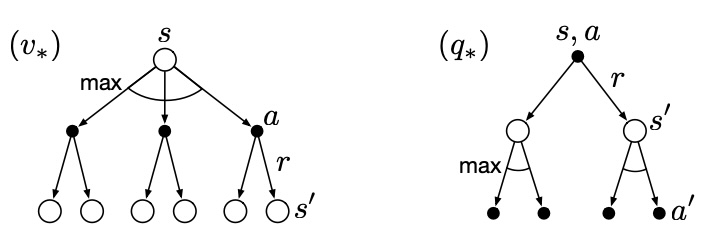
\includegraphics[width=\textwidth, trim=0 0 300 0, clip]{fig/backup_diagrams}}
	
	\begin{itemize} \normalsize
			\item Repite esta diagrama de respaldo desde los estados iniciales hasta los estados finales.
		\end{itemize}
	
\end{column}


\end{columns}

\end{frame}



%%%%%%%%%%%%%%%%%%%%%%%%%%%%%%%%%%
%%%%%%%%%%%%%%%%%%%%%%%%%%%%%%%%%%
% BIBLIOGRAFÍA
%%%%%%%%%%%%%%%%%%%%%%%%%%%%%%%%%%
%%%%%%%%%%%%%%%%%%%%%%%%%%%%%%%%%%


%%%%%%%%%%%%%%%%%%%%%%%%%%%%%%%%%%%%%%%%%%%%%%%%%%%%%%%%%%%%%%%%%%%%
%%%%%%%%%%%%%%%%%%%%%%%%%%%%%%%%%%%%%%%%%%%%%%%%%%%%%%%%%%%%%%%%%%%%

\section{Referencias}



% Redefinimos la apariencia
%\setbeamertemplate{headline}{}
%\setbeamertemplate{frametitle}{\vskip 0.5cm	\small{\textbf{\insertframetitle}}}
%\setbeamertemplate{footline}{}




% Mostramos la bibliografía
% \begin{frame}[allowframebreaks] %% Si ocupa más de una página
%\begin{frame}[allowframebreaks]{Referencias -} %% Si hay sólo una página

\begin{frame}{Referencias} %% Si hay sólo una página
\nocite{Sutton2018, silver2015lecture2, Hado2018Lecture3}

	% \vskip -5cm %% Para ajustar la distancia al comienzo	
	%\bibliography{references}	
	\printbibliography[heading=none]
\end{frame}    


		
%%%%%%%%%%%%%%%%%%%%%%%%%%%%%%%%%%
%%%%%%%%%%%%%%%%%%%%%%%%%%%%%%%%%%

\end{document}

%%%%%%%%%%%%%%%%%%%%%%%%%%%%%%%%%%
%%%%%%%%%%%%%%%%%%%%%%%%%%%%%%%%%%


\end{document}

